\documentclass{standalone}

\usepackage{TikzStyle}
\usepackage{mystyle}

\begin{document}
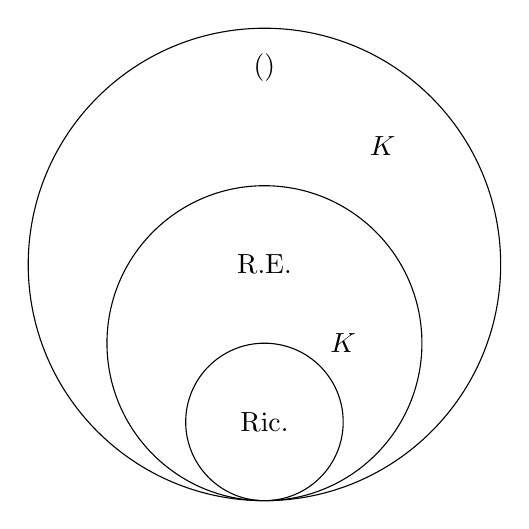
\begin{tikzpicture}
    \draw (0,0) circle [radius=3cm];
    \draw (0,-1) circle [radius=2cm];
    \draw (0,-2) circle [radius=1cm];
    \node at (0,2.5) {$\Parts(\Nat)$};
    \node at (1.5,1.5) {$\comp{K}$};
    \node at (0,0) {R.E.};
    \node at (1,-1) {$K$};
    \node at (0,-2) {Ric.};
\end{tikzpicture}
\end{document}
